%%% %%%%%%%%%%%%%%%%%%%%%%%%%%%% %%%
%%% Main Chapter 2 : Challenges  %%%
%%% %%%%%%%%%%%%%%%%%%%%%%%%%%%% %%%
\chapter{Experimente}
\label{chap:experiments}

In diesem Kapitel werden die einzelnen Experimente beschrieben, mit denen einige Neuerungen und auch Probleme der jeweiligen Version getestet werden können. Es soll später als Experimentierhandbuch verwendet werden können.

Jeder Abschnitt beschreit zunächst die notwendigen Vorbereitungen.
Anschließgend folgt aus eine Serie von Handlungsanweisungen. Danach folgt eine Erklärung, des erwarteten Verhalten und wie dies beobachtet werden kann.


%Was tun?
%Was beobachten?
%Aufbau?
%erwartetes Verhalten?

%Bspw. Übung: TSR durch Memory Abbild

%%%%%%%%%%%%%%%%%%%%%%%%%%%%%%%%%%%%%%%%%%%%%%%%%%%%%%%%%%%%%%%%%%%%%%%%%%%%%%%%%%%%%%%%%%%%%%%%%%%%%%%%%
\section{DOS 5.0}
%%%%%%%%%%%%%%%%%%%%%%%%%%%%%%%%%%%%%%%%%%%%%%%%%%%%%%%%%%%%%%%%%%%%%%%%%%%%%%%%%%%%%%%%%%%%%%%%%%%%%%%%%

	\subsection{TSR}

	Unter MS DOS konnten noch keine Anwendungen parallel ausgeführt werden. Insbesondere waren  Daemons oder Backgroundprozesse nicht vorgesehen.
	Um ein ähnliches Verhalten zu erzielen, konnte man sich mit sogenannten TSRs, "`Teminate and Stay Resident"'-Programmen behelfen\footnote{Eine hervorragende Einführung in die Programmierung und die Funktionsweise von TSRs befindet sich unter: \url{https://courses.engr.illinois.edu/ece390/books/artofasm/CH18/CH18-1.html\#HEADING1-3}}. 

	Eine sehr beliebte TSR war Sidekick, die unter anderm einen Taschenrechner und einen Kalender bereitstellte.

	\begin{figure}[h]
		\begin{center}
			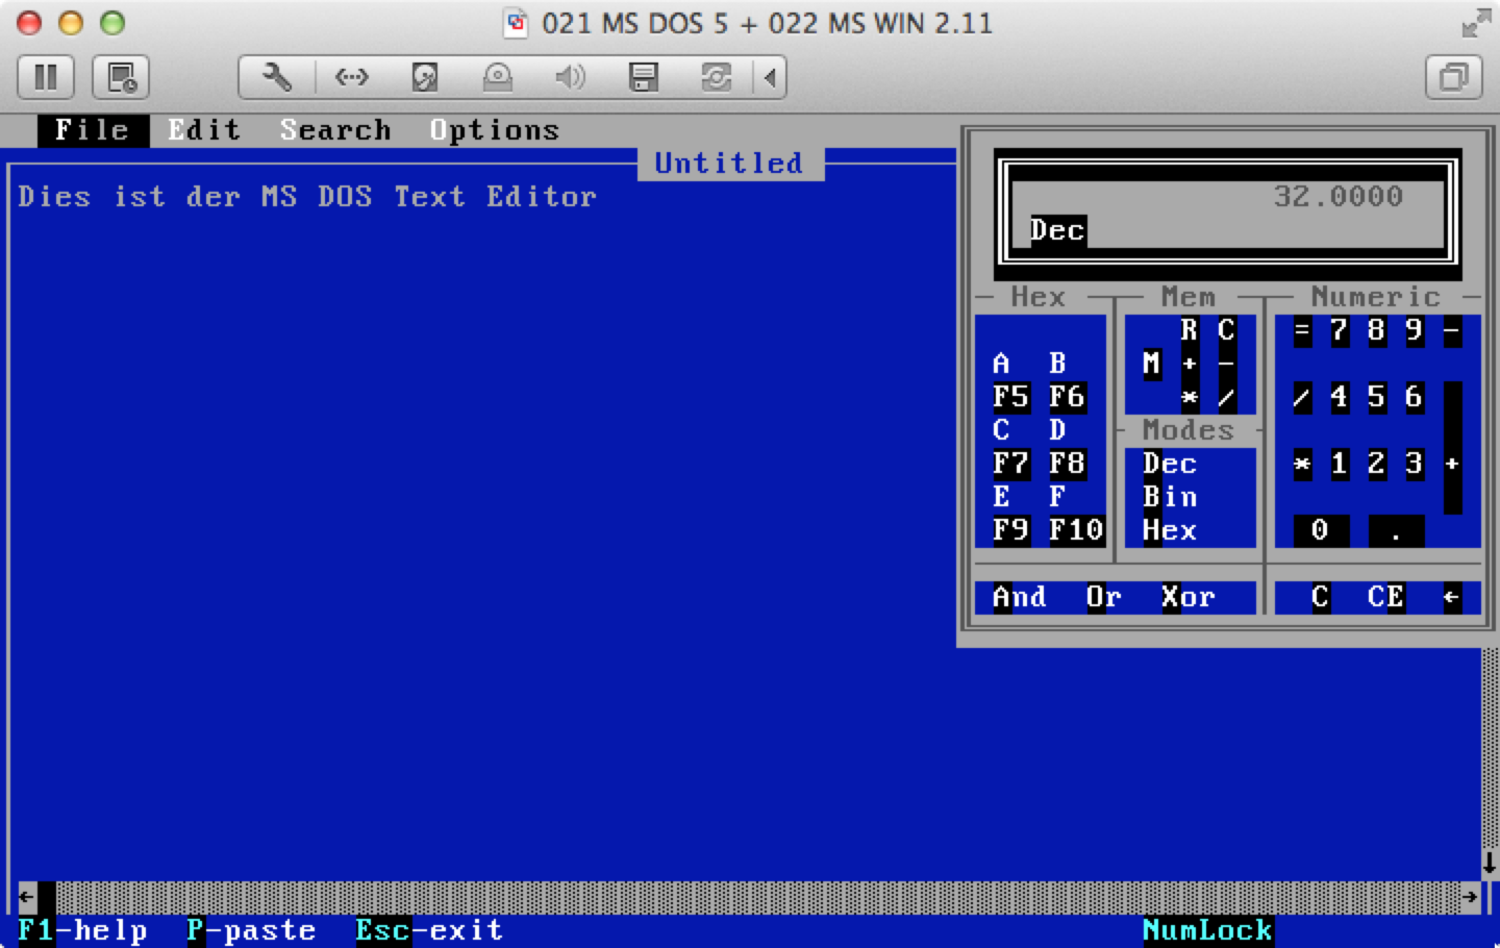
\includegraphics[width=0.8\textwidth]{img/dostsr}
			\caption{TSR-Taschenrechner vor dem DOS-Editor}
			\label{fig:screenshot-dostsr}
		\end{center}
	\end{figure}

	

	Starten 

	\subsection{Busy Waiting}
	
	Starten Sie die MS DOS VM und beobachten Sie ihr Verhalten.
	Wie viel CPU und Arbeitsspeicher verbraucht die VM und wie verändern sich die Parameter unter Last?

	Dosidle

	\subsection{DOS-Shell}

%%%%%%%%%%%%%%%%%%%%%%%%%%%%%%%%%%%%%%%%%%%%%%%%%%%%%%%%%%%%%%%%%%%%%%%%%%%%%%%%%%%%%%%%%%%%%%%%%%%%%%%%%
\section{Windows 2.11}
%%%%%%%%%%%%%%%%%%%%%%%%%%%%%%%%%%%%%%%%%%%%%%%%%%%%%%%%%%%%%%%%%%%%%%%%%%%%%%%%%%%%%%%%%%%%%%%%%%%%%%%%%

	\subsection{Koop. Multitasking}

%%%%%%%%%%%%%%%%%%%%%%%%%%%%%%%%%%%%%%%%%%%%%%%%%%%%%%%%%%%%%%%%%%%%%%%%%%%%%%%%%%%%%%%%%%%%%%%%%%%%%%%%%
\section{DOS 6.0}
%%%%%%%%%%%%%%%%%%%%%%%%%%%%%%%%%%%%%%%%%%%%%%%%%%%%%%%%%%%%%%%%%%%%%%%%%%%%%%%%%%%%%%%%%%%%%%%%%%%%%%%%%

	\subsection{Extended Memory}
	\subsection{DoubleSpace}

	Volume vs. DIR

%%%%%%%%%%%%%%%%%%%%%%%%%%%%%%%%%%%%%%%%%%%%%%%%%%%%%%%%%%%%%%%%%%%%%%%%%%%%%%%%%%%%%%%%%%%%%%%%%%%%%%%%%
\section{Windows 3.11}
%%%%%%%%%%%%%%%%%%%%%%%%%%%%%%%%%%%%%%%%%%%%%%%%%%%%%%%%%%%%%%%%%%%%%%%%%%%%%%%%%%%%%%%%%%%%%%%%%%%%%%%%%

	\subsection{Netzwerk}

	net use sub 
	ToDo für andere Infrastruktur mglw. zu Hause SMB Server und Kommandofolgen

	\subsection{Internet Explorer 5.0}

%%%%%%%%%%%%%%%%%%%%%%%%%%%%%%%%%%%%%%%%%%%%%%%%%%%%%%%%%%%%%%%%%%%%%%%%%%%%%%%%%%%%%%%%%%%%%%%%%%%%%%%%%
\section{Windows NT 3.51}
%%%%%%%%%%%%%%%%%%%%%%%%%%%%%%%%%%%%%%%%%%%%%%%%%%%%%%%%%%%%%%%%%%%%%%%%%%%%%%%%%%%%%%%%%%%%%%%%%%%%%%%%%

	\subsection{NTFS}
	Streams, Hidden files
	lange vs. kurze Dateinamen
	mehrere Namen pro File

	\subsection{VGA im User Mode}

%%%%%%%%%%%%%%%%%%%%%%%%%%%%%%%%%%%%%%%%%%%%%%%%%%%%%%%%%%%%%%%%%%%%%%%%%%%%%%%%%%%%%%%%%%%%%%%%%%%%%%%%%
\section{Windows NT 4.0 SP 6}
%%%%%%%%%%%%%%%%%%%%%%%%%%%%%%%%%%%%%%%%%%%%%%%%%%%%%%%%%%%%%%%%%%%%%%%%%%%%%%%%%%%%%%%%%%%%%%%%%%%%%%%%%

	\subsection{CSRSS}
	\subsection{EXEType}

%%%%%%%%%%%%%%%%%%%%%%%%%%%%%%%%%%%%%%%%%%%%%%%%%%%%%%%%%%%%%%%%%%%%%%%%%%%%%%%%%%%%%%%%%%%%%%%%%%%%%%%%%
\section{Windows 2000 Professional}
%%%%%%%%%%%%%%%%%%%%%%%%%%%%%%%%%%%%%%%%%%%%%%%%%%%%%%%%%%%%%%%%%%%%%%%%%%%%%%%%%%%%%%%%%%%%%%%%%%%%%%%%%

	\subsection{Active Directory}
	\subsection{EFS?}

